\documentclass{article}
\author{Grunda}
% Підключення додаткових пакетів
\usepackage[utf8]{inputenc} 
\usepackage[ukrainian]{babel}  
\usepackage{amsmath}  
\usepackage{graphicx} 
\usepackage{amsfonts} 
\usepackage{geometry}  
\usepackage{color}
\usepackage{listings}   % для відображення коду
\usepackage{color}      % для кольорів у коді
\usepackage{caption}    % для підписів до фігур/таблиць
\usepackage{hyperref}   % для гіперпосилань
\usepackage{tikz}
\usetikzlibrary{arrows.meta}
\geometry{left=2.5cm, right=2.5cm, top=2.5cm, bottom=2.5cm}

% Титульна сторінка
\title{Звіт до лабораторної роботи}
\author{Ярослав Грунда \\ Фі-21, ФТІ КПІ}
\date{\today}

\begin{document}

\maketitle

\tableofcontents  
\newpage

\section{Мета роботи}

Метою даної роботи є реалізація структури даних UnionFind за допомогою дерев та застосування її для алгоритму Краскала. 
Алгоритм Краскала використовується для побудови мінімального кістякового дерева неорієнтованого зваженого графа. 
У звіті розглянуто особливості реалізації алгоритму, а також проаналізовано його експериментальну продуктивність.

\section{Реалізація UnionFind}

\begin{itemize}
    \item \textbf{Клас Node}: кожен екземпляр має \texttt{value}, \texttt{parent} і \texttt{size}. 
    \item \textbf{Ініціалізація}: створюється масив з \texttt{n} кількістю об'єктів класу Node. Кожен Node має своє значення (\texttt{value} від 1 до \texttt{n} 
    відповідно до порядку створення) і є своїм власним батьком (є коренем дерева), розмір дерева при цьому дорівнює 1.
    \item \textbf{Операція Find}: виконує пошук кореня дерева для певного вузла (поки батько Node не є він самий, шукаємо батька Node). 
    Під час пошуку виконується компресія шляху: всі вузли, які знаходяться на шляху від початкового вузла до кореня, безпосередньо прикріпляються до кореня,
    тим самим зменшуючи глибину дерева для наступних пошуків. Це значно пришвидшує подальші операції пошуку.
    \item \textbf{Операція Union}: виконує об'єднання двох дерев, корені яких визначаються за допомогою операції \texttt{find}.
    Для оптимізації операції об'єднання застосовується \textbf{правило зваженого об'єднання}: менше дерево приєднується до більшого. 
    Це допомагає мінімізувати глибину дерев і зменшує час на виконання подальших операцій пошуку.
\end{itemize}

Операції в UnionFind мають такі складності:
\begin{itemize}
    \item Операція \texttt{find} — $O(\log n)$;
    \item Операція \texttt{union} — $O(\log n)$.
\end{itemize}

Алгоритм Крускала будує мінімальне кістякове дерево за допомогою таких кроків:
\begin{enumerate}
    \item Сортуємо ребра графа за вагою.
    \item Ініціалізуємо структуру Union-Find для $n$ вершин. Кожна вершина є коренем одного дерева.
    \item Ітеруємо через всі ребра в порядку зростання ваги.
    \item Перевіряємо, чи вершини $u$ і $v$ знаходяться у різних компонентах (не є з'єднаними) за допомогою методу find класу UnionFind 
    (output якого є коренем дерева, тому якщо корені однакові — це одна компонента). Якщо так, то:
    \begin{enumerate}
        \item Додаємо це ребро до мінімального кістякового дерева.
        \item Додаємо вагу цього ребра до загальної вартості MST.
    \end{enumerate}
    \item Завершуємо роботу, якщо кількість компонентів дорівнює 1.
\end{enumerate}

\section{Теоретична оцінка продуктивності алгоритму Крускала}
Теоретична складність алгоритму складається з:
\begin{itemize}
    \item Сортування ребер: $O(E \log E)$;
    \item Виконання операцій об'єднання і пошуку без компресії шляху: $O(V \log V)$;
    \item Виконання операцій об'єднання і пошуку з компресією шляху: $O(V \cdot G(V))$, де $G(V)$ — функція Акермана, яка для практичних значень є константою.
\end{itemize}

Можемо вважати складність виконання алгоритму без сортування — $O(V)$.

\section{Приклад виконання алгоритму Крускала}
\begin{figure}[ht]
    \centering
    \begin{minipage}{0.45\textwidth}
        \centering
        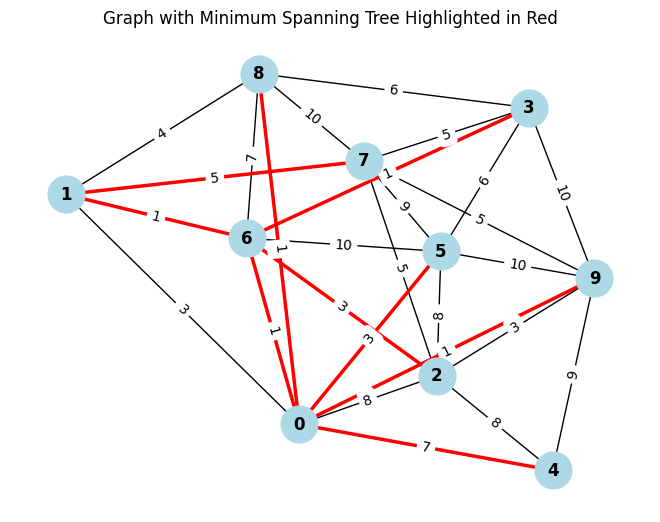
\includegraphics[width=\textwidth]{img/example1.png}
        \caption{Кількість вершин = 10, щільність = 0.7}
    \end{minipage}
    \hfill
    \begin{minipage}{0.45\textwidth}
        \centering
        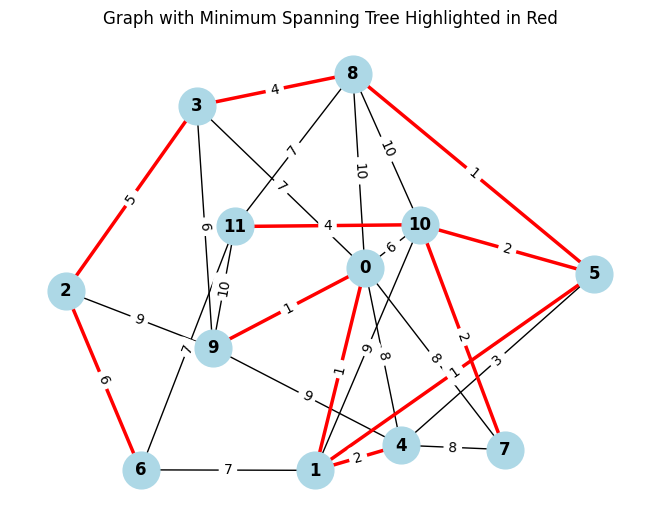
\includegraphics[width=\textwidth]{img/example2.png}
        \caption{Кількість вершин = 12, щільність = 0.4}
    \end{minipage}
\end{figure}

\section{Експериментальні дані алгоритму Крускала}
\begin{figure}[h!]
    \centering
    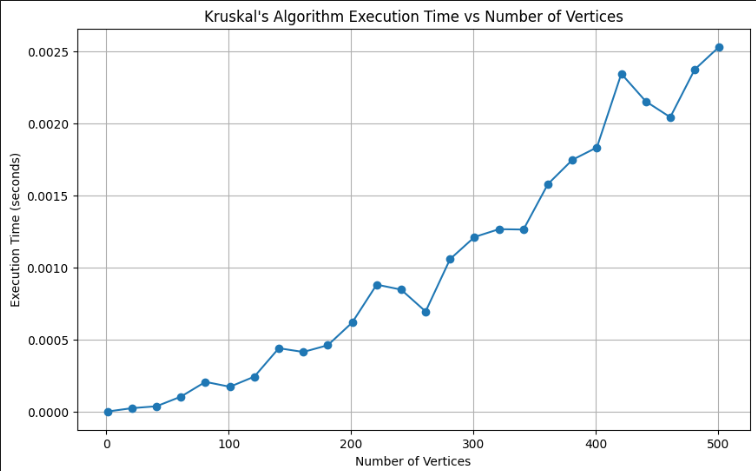
\includegraphics[width=0.8\textwidth]{img/image07.png}
    \caption{На рисунку з кроком 20 вершин показано залежність часу виконання алгоритму Крускала (з компресією шляху) 
    від кількості вершин графа при щільності 0.7. На кожну кількість вершин взято середній час 1000 експериментів.}
\end{figure}
\newpage
\begin{figure}[h!]
    \centering
    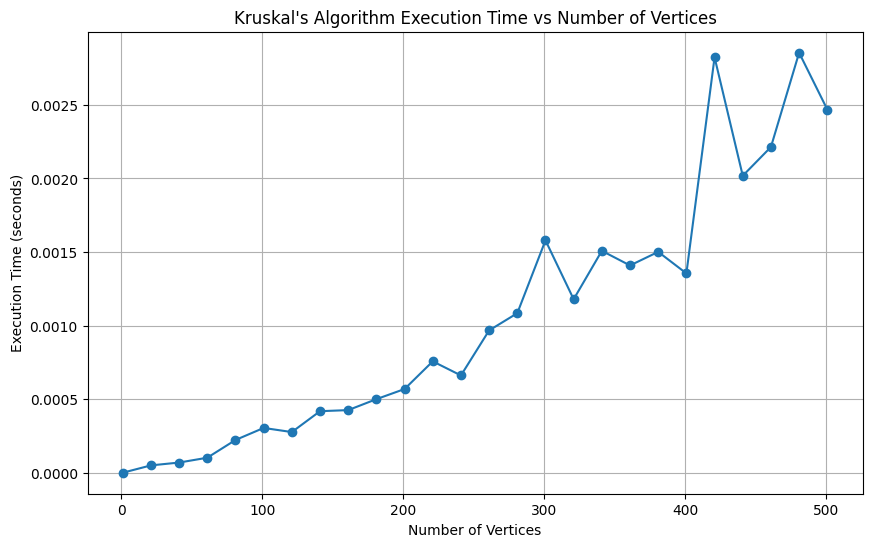
\includegraphics[width=0.8\textwidth]{img/image05.png}
    \caption{На рисунку з кроком 20 вершин показано залежність часу виконання алгоритму Крускала (з компресією шляху) 
    від кількості вершин графа при щільності 0.5. На кожну кількість вершин взято середній час 1000 експериментів.}
\end{figure}

\begin{figure}[h!]
    \centering
    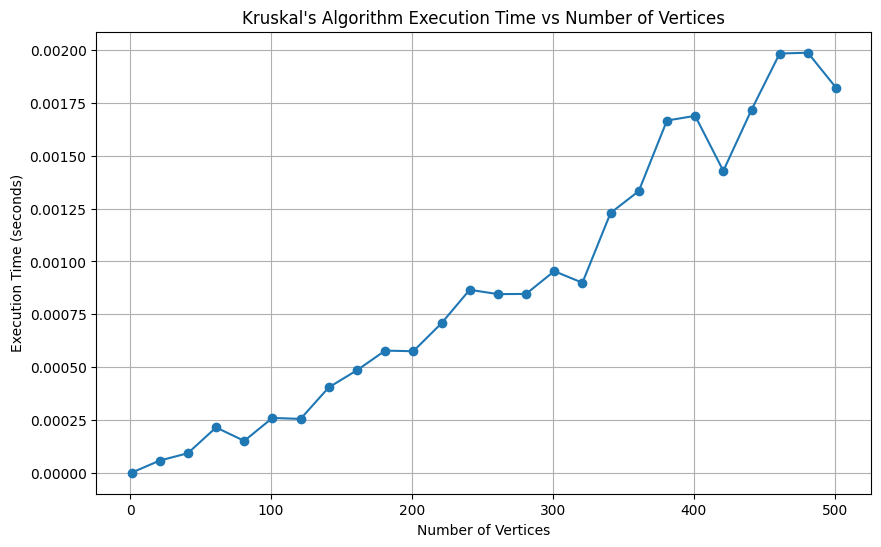
\includegraphics[width=0.8\textwidth]{img/image02.png}
    \caption{На рисунку з кроком 20 вершин показано залежність часу виконання алгоритму Крускала (з компресією шляху) 
    від кількості вершин графа при щільності 0.2. На кожну кількість вершин взято середній час 1000 експериментів.}
\end{figure}

Бачимо досить лінійну залежність часу, з деякими скачками, які можна пояснити характеристиками згенерованих графів. 
Цей результат відповідає теоретичній оцінці $O(V)$.

Для більш детальної інформації, будь ласка, відвідайте наступний ресурс: \href{https://github.com/gre1wy/AppliedAlgorithms/tree/main/lab4}{Перейти до репозиторію}.
\end{document}